\documentclass[12pt,a4paper]{article}

% ── Packages ──────────────────────────────────────────────────────────────────
\usepackage[a4paper, margin=2.5cm]{geometry}
\usepackage{fontenc}
\usepackage{inputenc}
\usepackage{microtype}
\usepackage{lmodern}
\usepackage{xcolor}
\usepackage{graphicx}
\usepackage{booktabs}
\usepackage{longtable}
\usepackage{tabularx}
\usepackage{multirow}
\usepackage{array}
\usepackage{listings}
\usepackage{amsmath}
\usepackage{amssymb}
\usepackage{hyperref}
\usepackage{fancyhdr}
\usepackage{titlesec}
\usepackage{tcolorbox}
\usepackage{enumitem}
\usepackage{tikz}
\usepackage{float}
\usepackage{caption}
\usepackage{subcaption}
\usepackage{mdframed}
\usepackage{parskip}
\usepackage{setspace}
\usepackage{csquotes}
\usepackage{nameref}

\usetikzlibrary{shapes.geometric, arrows.meta, positioning, fit, backgrounds, calc}

% ── Colours ───────────────────────────────────────────────────────────────────
\definecolor{prahariblue}{RGB}{30, 64, 175}
\definecolor{praharired}{RGB}{185, 28, 28}
\definecolor{praharigreen}{RGB}{21, 128, 61}
\definecolor{prahariyellow}{RGB}{161, 98, 7}
\definecolor{praharigray}{RGB}{75, 85, 99}
\definecolor{codebg}{RGB}{245, 245, 245}
\definecolor{codeframe}{RGB}{200, 200, 200}
\definecolor{noteblue}{RGB}{219, 234, 254}
\definecolor{noteblueborder}{RGB}{147, 197, 253}
\definecolor{warnbg}{RGB}{254, 243, 199}
\definecolor{warnborder}{RGB}{251, 191, 36}

% ── Hyperref ──────────────────────────────────────────────────────────────────
\hypersetup{
    colorlinks=true,
    linkcolor=prahariblue,
    urlcolor=prahariblue,
    citecolor=praharired,
    pdftitle={PRAHARI — Technical Report},
    pdfauthor={Soham Banerjee},
    pdfsubject={AI-Powered Tender Intelligence Platform},
}

% ── Headers / Footers ─────────────────────────────────────────────────────────
\pagestyle{fancy}
\fancyhf{}
\fancyhead[L]{\small\color{praharigray}PRAHARI — Technical Report}
\fancyhead[R]{\small\color{praharigray}AI For Bharat · Soham Banerjee}
\fancyfoot[C]{\small\color{praharigray}\thepage}
\renewcommand{\headrulewidth}{0.4pt}

% ── Section formatting ────────────────────────────────────────────────────────
\titleformat{\section}{\large\bfseries\color{prahariblue}}{{\thesection}}{1em}{}[\color{prahariblue}\titlerule]
\titleformat{\subsection}{\normalsize\bfseries\color{praharigray}}{{\thesubsection}}{1em}{}
\titleformat{\subsubsection}{\normalsize\itshape\color{praharigray}}{{\thesubsubsection}}{1em}{}

% ── Code listings ─────────────────────────────────────────────────────────────
\lstdefinestyle{pythonstyle}{
    language=Python,
    backgroundcolor=\color{codebg},
    frame=single,
    rulecolor=\color{codeframe},
    basicstyle=\ttfamily\small,
    keywordstyle=\color{prahariblue}\bfseries,
    commentstyle=\color{praharigray}\itshape,
    stringstyle=\color{praharigreen},
    numberstyle=\tiny\color{praharigray},
    numbers=left,
    numbersep=6pt,
    breaklines=true,
    captionpos=b,
    showstringspaces=false,
    tabsize=4,
}

\lstdefinestyle{sqlstyle}{
    language=SQL,
    backgroundcolor=\color{codebg},
    frame=single,
    rulecolor=\color{codeframe},
    basicstyle=\ttfamily\small,
    keywordstyle=\color{praharired}\bfseries,
    commentstyle=\color{praharigray}\itshape,
    stringstyle=\color{praharigreen},
    breaklines=true,
    showstringspaces=false,
    tabsize=4,
}

\lstdefinestyle{bashstyle}{
    language=bash,
    backgroundcolor=\color{codebg},
    frame=single,
    rulecolor=\color{codeframe},
    basicstyle=\ttfamily\small,
    keywordstyle=\color{prahariblue},
    stringstyle=\color{praharigreen},
    commentstyle=\color{praharigray}\itshape,
    breaklines=true,
    showstringspaces=false,
}

% ── Custom boxes ──────────────────────────────────────────────────────────────
\tcbuselibrary{skins, breakable}

\newtcolorbox{infobox}[1][]{
    colback=noteblue, colframe=noteblueborder,
    fonttitle=\bfseries\small,
    title=#1, boxrule=0.5pt, arc=3pt,
    left=6pt, right=6pt, top=4pt, bottom=4pt,
}

\newtcolorbox{warnbox}[1][]{
    colback=warnbg, colframe=warnborder,
    fonttitle=\bfseries\small,
    title=#1, boxrule=0.5pt, arc=3pt,
    left=6pt, right=6pt, top=4pt, bottom=4pt,
}

\newtcolorbox{guaranteebox}{
    colback=white, colframe=prahariblue,
    fonttitle=\bfseries,
    title=Core Guarantee, boxrule=1pt, arc=4pt,
    left=8pt, right=8pt, top=6pt, bottom=6pt,
}

% ── Spacing ───────────────────────────────────────────────────────────────────
\setlength{\parskip}{6pt}
\setlength{\parindent}{0pt}

% ══════════════════════════════════════════════════════════════════════════════
\begin{document}
% ══════════════════════════════════════════════════════════════════════════════

% ── Title Page ────────────────────────────────────────────────────────────────
\begin{titlepage}
\centering
\vspace*{2cm}

{\color{prahariblue}\rule{\linewidth}{2pt}}
\vspace{0.5cm}

{\Huge\bfseries\color{prahariblue} PRAHARI}\\[0.3cm]
{\large\color{praharigray}\textit{प्रहरी}}\\[0.3cm]
{\LARGE\bfseries Proactive Requisition Audit \&}\\[0.2cm]
{\LARGE\bfseries Honest AI for Righteous Integrity}\\[0.5cm]

{\color{prahariblue}\rule{\linewidth}{1pt}}
\vspace{0.8cm}

{\large\bfseries AI-Powered Tender Intelligence Platform}\\[0.2cm]
{\large for CRPF Procurement Evaluation}

\vspace{1.2cm}

\begin{tcolorbox}[colback=noteblue, colframe=noteblueborder, boxrule=0.5pt, arc=4pt,
    left=12pt, right=12pt, top=8pt, bottom=8pt, width=0.82\linewidth]
\centering
\textbf{Problem Statement:} PS-1652 \\[4pt]
\small Develop an AI-based system to automate the evaluation of tender documents for
Central Reserve Police Force (CRPF) procurement with transparency, auditability,
and bias detection.
\end{tcolorbox}

\vspace{1.2cm}

\begin{tabular}{ll}
\textbf{Author}     & Soham Banerjee \\[4pt]
\textbf{Event}      & AI For Bharat \\[4pt]
\textbf{Domain}     & Government Procurement \& Tender Evaluation \\[4pt]
\textbf{Category}   & Software \\[4pt]
\textbf{Stack}      & FastAPI $\cdot$ PostgreSQL $\cdot$ React 18 $\cdot$ Gemini 2.5 Flash \\[4pt]
\textbf{Date}       & May 2026 \\
\end{tabular}

\vfill

{\color{prahariblue}\rule{\linewidth}{1pt}}\\[0.3cm]
{\small\color{praharigray}This document is the official technical report for the PRAHARI system,
submitted for AI For Bharat by Soham Banerjee.}

\end{titlepage}

% ── Table of Contents ─────────────────────────────────────────────────────────
\tableofcontents
\newpage

% ══════════════════════════════════════════════════════════════════════════════
\section*{Abstract}
\addcontentsline{toc}{section}{Abstract}
% ══════════════════════════════════════════════════════════════════════════════

PRAHARI (\textit{प्रहरी} — Hindi for \enquote{guardian}) is a full-stack, production-ready
AI platform that transforms government tender evaluation from a months-long manual
process into a transparent, auditable, and bias-resistant pipeline completing in
under ten minutes.

The system implements a nine-stage AI evaluation pipeline powered by Google Gemini
2.5 Flash multimodal inference. It extracts eligibility criteria from Notice Inviting
Tender (NIT) documents, benchmarks thresholds against market data to detect
threshold-rigging, scores bidder documents for authenticity, evaluates every criterion
with evidence citations linked to exact PDF pages, performs cross-bidder collusion
detection, applies differential privacy ($\varepsilon$-DP) to aggregate analytics,
routes borderline cases to human review, and generates SHA-256 tamper-proof PDF audit
reports with officer digital sign-off.

PRAHARI supports Indic script OCR (Hindi, Tamil, Urdu, Marathi) via Gemini multimodal,
making it the first system to address the language accessibility gap in Indian
government procurement evaluation. The backend is built on FastAPI with PostgreSQL
persistence, JWT authentication, and rate limiting. The frontend is React~18 with
TypeScript and includes an in-browser PDF viewer with fuzzy text highlighting for
evidence traceability. The system is fully containerised, CI-tested, and deployable
on Render (backend) and Vercel (frontend) with a single configuration file each.

\textbf{Keywords:} tender evaluation, AI procurement, government transparency, differential privacy,
collusion detection, Gemini multimodal, FastAPI, CRPF.

\newpage

% ══════════════════════════════════════════════════════════════════════════════
\section{Introduction}
% ══════════════════════════════════════════════════════════════════════════════

\subsection{Background}

India's government procurement ecosystem represents approximately \textbf{20\% of GDP}
--- roughly \rupee40 lakh crore annually. The Central Reserve Police Force (CRPF), as
one of India's largest central paramilitary forces, conducts over \textbf{500 tenders
per year} for mission-critical equipment including bullet-resistant jackets, vehicles,
communication systems, and infrastructure.

The current evaluation process is entirely manual: committees of five to eight
officers read hundreds of pages per bidder, score eligibility criteria subjectively,
and compile results without systematic audit trails. A major tender can take three to
six months to evaluate, requiring 200--400 person-hours per evaluation cycle.

\subsection{Motivation}

The Comptroller and Auditor General (CAG) of India reported \textbf{\rupee3.5 lakh crore}
in procurement-related financial irregularities over five years. Approximately one in
four procurement decisions is challenged in court, often because the evaluation
process lacks reproducibility. More critically, CRPF personnel are sometimes deployed
without required protective equipment because procurement delays exceeded the
operational timeline.

The problem is not a shortage of qualified evaluators — it is a process problem.
Manual evaluation of multi-hundred-page tender documents is inherently error-prone,
unscalable, and difficult to audit. Evaluators miss criteria, apply inconsistent
thresholds, and have no way to detect coordinated bidding between supposedly
independent vendors.

\subsection{Scope}

This report describes the design, implementation, and evaluation of PRAHARI — a
system that addresses the above challenges through AI-assisted evaluation while
maintaining human officer authority over all final decisions. The system is designed
for deployment within CRPF procurement operations and is architected to scale across
all seven Central Armed Police Forces (CAPFs).

% ══════════════════════════════════════════════════════════════════════════════
\section{Problem Statement}
% ══════════════════════════════════════════════════════════════════════════════

We identify five root causes of failure in the current procurement evaluation process:

\begin{enumerate}[leftmargin=*, label=\textbf{P\arabic*.}]

\item \textbf{Manual criterion extraction and scoring.}
Evaluators read NIT documents and manually identify criteria, often missing
implicit requirements embedded in dense legal language. No two evaluators produce
identical criterion lists from the same document.

\item \textbf{No evidence traceability.}
Evaluation verdicts are recorded as binary (pass/fail) with no citation of the
specific page, paragraph, or sentence in the bidder's document that supported the
verdict. This makes audit and RTI responses impossible to automate.

\item \textbf{Absence of forgery and authenticity checks.}
Financial documents (CA-certified balance sheets, bank statements, turnover
certificates) submitted by bidders are not systematically verified for
authenticity. Metadata anomalies, digital signature gaps, and font embedding
inconsistencies are ignored.

\item \textbf{No collusion detection.}
Multiple bidders may coordinate their bids to create the appearance of competition
while pre-agreeing on outcomes. The current process has no mechanism to detect
identical document sections, price coordination patterns, or shared infrastructure
(email domains, IP addresses).

\item \textbf{Threshold manipulation by procurement officers.}
Eligibility thresholds are set by the procuring entity. A corrupt officer can set
a turnover threshold or delivery timeline specifically calibrated to include a
favoured vendor and exclude competitors. No mechanism exists to flag statistically
anomalous criteria before the tender is published.

\end{enumerate}

% ══════════════════════════════════════════════════════════════════════════════
\section{Solution Overview}
% ══════════════════════════════════════════════════════════════════════════════

PRAHARI addresses all five root causes through a structured pipeline with
mathematically grounded safeguards.

\begin{guaranteebox}
No bidder is automatically assigned a \texttt{Not\_Eligible} verdict unless the AI
model reports $\geq 90\%$ confidence AND the criterion is flagged as mandatory.
Everything below that threshold is routed to a human review queue. Optional criteria
failures never trigger disqualification.
\end{guaranteebox}

\subsection{Three-Role Architecture}

The system serves three distinct user roles with separate interfaces and capabilities:

\begin{table}[H]
\centering
\begin{tabularx}{\linewidth}{@{}lX@{}}
\toprule
\textbf{Role} & \textbf{PRAHARI Capabilities} \\
\midrule
Procurement Officer &
    Criteria extraction, bidder registration, document upload, evaluation
    trigger, verdict review, override with justification, officer digital
    sign-off, PDF report download \\[6pt]
Auditor &
    Read-only access to SHA-256 hashed audit trail, override history,
    sign-off records, and full event timeline for any tender \\[6pt]
Bidder (self-check) &
    Pre-submission portal: upload own documents against active tender
    criteria and receive a preliminary eligibility assessment before
    the official deadline \\
\bottomrule
\end{tabularx}
\caption{Role-based capabilities in PRAHARI}
\end{table}

% ══════════════════════════════════════════════════════════════════════════════
\section{System Architecture}
% ══════════════════════════════════════════════════════════════════════════════

\subsection{High-Level Architecture}

\begin{figure}[H]
\centering
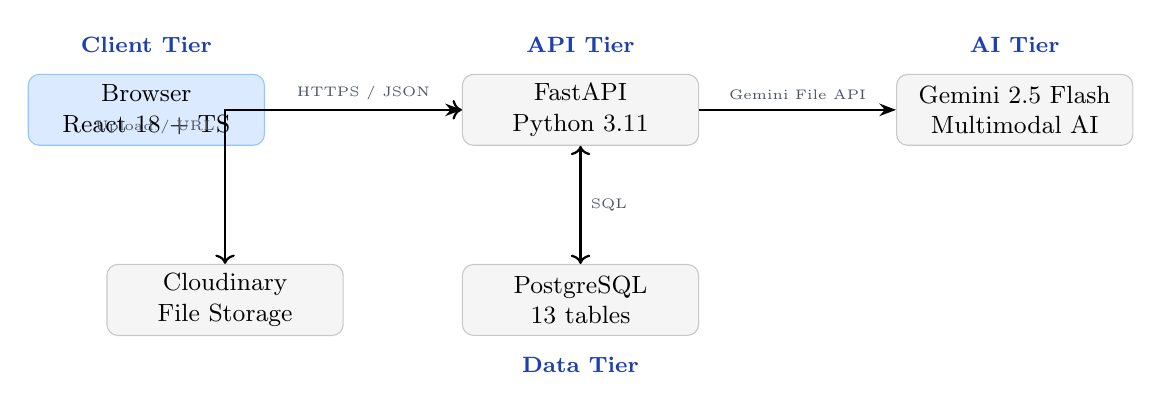
\begin{tikzpicture}[
    box/.style={rectangle, rounded corners=4pt, draw, minimum width=3cm,
                minimum height=0.9cm, align=center, font=\small},
    arrow/.style={-{Stealth[length=6pt]}, thick},
    label/.style={font=\tiny\color{praharigray}},
]

% Client tier
\node[box, fill=noteblue, draw=noteblueborder] (browser) {Browser\\React 18 + TS};

% API tier
\node[box, fill=codebg, draw=codeframe, right=2.5cm of browser] (api)
    {FastAPI\\Python 3.11};

% AI tier
\node[box, fill=codebg, draw=codeframe, right=2.5cm of api] (gemini)
    {Gemini 2.5 Flash\\Multimodal AI};

% Data tier — below API
\node[box, fill=codebg, draw=codeframe, below=1.5cm of api] (pg)
    {PostgreSQL\\13 tables};
\node[box, fill=codebg, draw=codeframe, left=1.5cm of pg] (cloud)
    {Cloudinary\\File Storage};

% Arrows
\draw[arrow] (browser) -- node[above, label]{HTTPS / JSON} (api);
\draw[arrow] (api) -- node[above, label]{Gemini File API} (gemini);
\draw[arrow, <->] (api) -- node[right, label]{SQL} (pg);
\draw[arrow, <->] (api) -| node[below left, label]{Upload / URL} (cloud);

% Labels
\node[above=0.15cm of browser, font=\footnotesize\bfseries\color{prahariblue}]
    {Client Tier};
\node[above=0.15cm of api, font=\footnotesize\bfseries\color{prahariblue}]
    {API Tier};
\node[above=0.15cm of gemini, font=\footnotesize\bfseries\color{prahariblue}]
    {AI Tier};
\node[below=0.15cm of pg, font=\footnotesize\bfseries\color{prahariblue}]
    {Data Tier};

\end{tikzpicture}
\caption{PRAHARI three-tier system architecture}
\end{figure}

\subsection{Technology Stack}

\begin{table}[H]
\centering
\begin{tabularx}{\linewidth}{@{}llX@{}}
\toprule
\textbf{Layer} & \textbf{Technology} & \textbf{Rationale} \\
\midrule
AI Inference       & Google Gemini 2.5 Flash      & Multimodal; Indic language OCR; File API for large docs \\
Backend Framework  & FastAPI 0.110 (Python 3.11)  & Async ASGI; OpenAPI auto-docs; easy Gemini SDK integration \\
Database           & PostgreSQL 14                & ACID; JSONB for verdict payloads; row-level audit trail \\
File Storage       & Cloudinary                   & CDN-backed; signed URLs; no storage limits on eval plan \\
Frontend           & React 18 + TypeScript + Vite & Type-safe; component model suits complex evaluation UI \\
Styling            & Tailwind CSS + shadcn/ui     & Accessible; dark-mode; rapid iteration \\
PDF Rendering      & react-pdf (pdfjs-dist)       & Client-side; text layer access for exact highlighting \\
Authentication     & PyJWT + bcrypt               & Stateless JWT; HS256; bcrypt cost factor 12 \\
Rate Limiting      & slowapi                      & Per-IP per-endpoint limits; Gemini cost protection \\
Containerisation   & Docker multi-stage           & Minimal production image; non-root user \\
CI/CD              & GitHub Actions               & 3-job pipeline: TypeScript, Python, Docker \\
Privacy            & diffprivlib (custom)         & Laplace mechanism; $\varepsilon$-DP budget tracking \\
\bottomrule
\end{tabularx}
\caption{Complete technology stack}
\end{table}

% ══════════════════════════════════════════════════════════════════════════════
\section{The Nine-Stage Evaluation Pipeline}
% ══════════════════════════════════════════════════════════════════════════════

PRAHARI processes each tender through nine sequential stages. Stages 1--3 operate
on the tender document itself; Stages 4--6 operate on bidder submissions; Stages
7--9 operate at the tender level after all bidders are evaluated.

\subsection{Stage 1: Criteria Extraction}

\textbf{Input:} NIT / tender PDF or DOCX \\
\textbf{Output:} Structured JSON list of criteria with thresholds, weights, and mandatory flags

The tender document is uploaded to Gemini via the File API (bypassing per-request
token limits). A structured prompt instructs Gemini to extract all eligibility criteria
and return a JSON array with fields: \texttt{id}, \texttt{description},
\texttt{threshold}, \texttt{unit}, \texttt{is\_mandatory}, \texttt{weight}.

\begin{lstlisting}[style=pythonstyle, caption={Criteria extraction prompt structure}]
EXTRACTION_PROMPT = """
You are a government procurement analyst. Read the attached NIT document
and extract every eligibility criterion into a JSON array.

For each criterion include:
- id: sequential identifier (C001, C002, ...)
- description: plain-language description
- threshold: numeric or textual threshold value
- unit: unit of measurement (INR, years, count, etc.)
- is_mandatory: true if disqualifying when failed, false if preferred
- weight: relative importance 0.0 to 1.0

Return ONLY valid JSON. No markdown, no explanation.
"""
\end{lstlisting}

\subsection{Stage 2: Market Benchmark Validation}

\textbf{Input:} Extracted criteria thresholds \\
\textbf{Output:} Benchmark report with anomaly flags

Each numeric threshold is compared against sector-average data maintained in
\texttt{backend/market\_benchmark.py}. Thresholds that are statistically anomalous
(too high, too narrow, or suspiciously specific) are flagged as potential
threshold-rigging signals. This stage runs \textit{before any bidder is registered},
auditing the procurement officer's own document.

\begin{infobox}[Threshold-Rigging Detection]
A turnover threshold of exactly \rupee47.3~crore where the sector average is
\rupee12~crore, and only one known vendor has exactly that turnover, is a
statistical red flag. PRAHARI surfaces this to senior approvers before the
tender opens for bidding.
\end{infobox}

\subsection{Stage 3: Document Authenticity Scoring}

\textbf{Input:} Bidder uploaded documents \\
\textbf{Output:} Authenticity score (0--100) with anomaly list

Each document is analysed for:
\begin{itemize}
\item PDF metadata anomalies (creation date, software, author field)
\item Digital signature presence and chain validity
\item Font embedding inconsistencies (common in spliced forgeries)
\item Image-over-text layers (scanned originals pasted over digital certificates)
\end{itemize}

\subsection{Stage 4: Bidder Ingestion and Document Normalisation}

\textbf{Input:} Uploaded files (PDF, DOCX, images, scanned pages) \\
\textbf{Output:} Normalised text representation for Gemini

The \texttt{document\_converter.py} module routes each file through the appropriate
normalisation path:

\begin{verbatim}
Upload
  ├─ .docx            → python-docx → plain text
  ├─ .pdf (digital)   → Gemini File API (native)
  ├─ .pdf (scanned)   → Gemini File API (multimodal OCR)
  └─ .jpg / .png      → Gemini File API (vision)
\end{verbatim}

Gemini's multimodal capability provides Indic script OCR for documents in Hindi,
Tamil, Urdu, and Marathi --- languages that no existing procurement system
handles automatically.

\subsection{Stage 5: Criterion-by-Criterion Evaluation}

\textbf{Input:} Normalised bidder document + criteria list \\
\textbf{Output:} Per-criterion verdict with confidence, evidence quote, and page reference

For each criterion, Gemini is asked to:
\begin{enumerate}
\item Find the relevant section in the bidder's document
\item Extract the specific value claimed
\item Compare it to the threshold
\item Return a structured verdict
\end{enumerate}

\begin{lstlisting}[style=pythonstyle, caption={Verdict structure returned by Gemini}]
{
  "criterion_id": "C001",
  "verdict": "Eligible",          # Eligible | Not_Eligible | Manual_Review
  "confidence": 0.94,             # 0.0 – 1.0
  "extracted_value": "18.48 Cr",
  "threshold": "10 Cr",
  "evidence_quote": "Average annual turnover for FY 2021-22 to FY 2023-24
                     as certified by CA: INR 18,48,00,000",
  "page_reference": 12
}
\end{lstlisting}

The \textbf{confidence threshold rule} is enforced in Python, not in the prompt:
if \texttt{verdict == "Not\_Eligible"} and \texttt{confidence < 0.90} and
\texttt{is\_mandatory == True}, the verdict is overridden to \texttt{Manual\_Review}.

\subsection{Stage 6: Collusion Detection}

\textbf{Input:} All bidder documents for a tender \\
\textbf{Output:} Collusion risk report with flagged bidder pairs

Cross-bidder analysis runs four checks:

\begin{table}[H]
\centering
\begin{tabularx}{\linewidth}{@{}lX@{}}
\toprule
\textbf{Check} & \textbf{Method} \\
\midrule
Identical text sections &
    SHA-256 hashes of overlapping sliding windows across document pairs \\[4pt]
Price coordination &
    Statistical analysis of bid prices for suspicious clustering
    (prices within 0.5\% of each other) \\[4pt]
Shared infrastructure &
    Email domain, registered address, and phone prefix matching across
    bidder registration data \\[4pt]
Complementary bidding &
    Detection of patterns where one bidder always scores just above
    mandatory thresholds while others score just below \\
\bottomrule
\end{tabularx}
\caption{Collusion detection checks}
\end{table}

\subsection{Stage 7: Differential Privacy Analytics}

\textbf{Input:} Raw evaluation results \\
\textbf{Output:} Privacy-preserving aggregate statistics

Aggregate statistics (average confidence per criterion, score distribution,
criterion pass rates) are computed with Laplace-mechanism differential privacy:

\begin{equation}
\tilde{f}(D) = f(D) + \text{Lap}\!\left(\frac{\Delta f}{\varepsilon}\right)
\end{equation}

where $\Delta f$ is the global sensitivity of the query and $\varepsilon$ is the
privacy budget. A per-project $\varepsilon$-budget is tracked in the database;
once exhausted, further aggregate queries are rejected. This ensures that
individual bidder data cannot be reverse-engineered from repeated queries.

\subsection{Stage 8: Human Review and Officer Sign-Off}

\textbf{Input:} Evaluation results with \texttt{Manual\_Review} verdicts \\
\textbf{Output:} Officer-reviewed verdicts with justifications; digital sign-off record

Officers can override any \texttt{Manual\_Review} verdict (upgrade to
\texttt{Eligible} or downgrade to \texttt{Not\_Eligible}) with a mandatory
free-text justification. Each override is stored in the audit trail with a
timestamp, officer identity, and original AI verdict.

When all manual reviews are resolved, the officer signs off the evaluation using
a JWT-authenticated endpoint. The sign-off is recorded with the officer name,
timestamp, and tender reference. \textbf{Sign-off is blocked if any
\texttt{Manual\_Review} verdicts remain unresolved.}

\subsection{Stage 9: Audit Report Generation}

\textbf{Input:} Signed-off evaluation record \\
\textbf{Output:} PDF audit report

The report is generated using WeasyPrint from a Jinja2 HTML template and includes:
\begin{itemize}
\item Tender reference, criteria summary, and benchmark results
\item Verdicts matrix (all bidders × all criteria) with confidence scores
\item Authenticity scores and anomaly summaries per bidder
\item Collusion detection findings
\item Complete override history (AI verdict → officer verdict + justification)
\item Differential privacy analytics section
\item Officer digital sign-off block with timestamp
\item SHA-256 report hash for tamper detection
\end{itemize}

% ══════════════════════════════════════════════════════════════════════════════
\section{Database Schema}
% ══════════════════════════════════════════════════════════════════════════════

PRAHARI uses a PostgreSQL relational database with 13 tables. All tables use
\texttt{SERIAL} primary keys and \texttt{TIMESTAMP DEFAULT NOW()} for creation times.

\begin{longtable}{@{}p{3.2cm}p{2.8cm}p{6.5cm}@{}}
\toprule
\textbf{Table} & \textbf{Key Columns} & \textbf{Purpose} \\
\midrule
\endhead
\texttt{users} &
    \texttt{id, username,} \newline \texttt{password\_hash, role} &
    Authentication table. \texttt{role} is \texttt{admin} or \texttt{user}.
    Passwords hashed with bcrypt (cost 12). \\[6pt]

\texttt{projects} &
    \texttt{id, name, state,} \newline \texttt{signed\_by, signed\_at} &
    Top-level tender records. \texttt{state} tracks workflow status.
    \texttt{signed\_by / signed\_at} populated on officer sign-off. \\[6pt]

\texttt{dprs} &
    \texttt{id, project\_id,} \newline \texttt{file\_url, processed} &
    Uploaded tender NIT documents. Cloudinary URL stored; full text
    cached for re-evaluation without re-upload. \\[6pt]

\texttt{criteria} &
    \texttt{id, project\_id,} \newline \texttt{description, threshold,} \newline
    \texttt{is\_mandatory, weight} &
    Extracted eligibility criteria. One row per criterion per project. \\[6pt]

\texttt{compliance\_weights} &
    \texttt{project\_id,} \newline \texttt{criterion\_id, weight} &
    Officer-adjustable per-criterion weights. Overrides the AI-extracted
    default weights when set. \\[6pt]

\texttt{bidders} &
    \texttt{id, project\_id,} \newline \texttt{name, gstin, pan} &
    Registered bidder entities with identity verification fields. \\[6pt]

\texttt{bidder\_documents} &
    \texttt{id, bidder\_id,} \newline \texttt{file\_url, doc\_type} &
    Uploaded bidder qualification documents. Multiple documents
    per bidder are supported. \\[6pt]

\texttt{verdicts} &
    \texttt{id, bidder\_id,} \newline \texttt{criterion\_id, verdict,} \newline
    \texttt{confidence, evidence\_quote,} \newline \texttt{page\_reference} &
    AI-generated per-criterion verdicts. \texttt{verdict} is one of
    \texttt{Eligible}, \texttt{Not\_Eligible}, \texttt{Manual\_Review}. \\[6pt]

\texttt{overrides} &
    \texttt{id, verdict\_id,} \newline \texttt{officer, old\_verdict,} \newline
    \texttt{new\_verdict, justification} &
    Human override records. Stores both original AI verdict and
    officer replacement for full audit traceability. \\[6pt]

\texttt{audit\_events} &
    \texttt{id, project\_id,} \newline \texttt{event\_type, payload,} \newline
    \texttt{sha256\_hash} &
    Immutable event log. Every AI call, override, sign-off, and
    report download is recorded with a SHA-256 payload hash. \\[6pt]

\texttt{collusion\_reports} &
    \texttt{id, project\_id,} \newline \texttt{report\_json} &
    JSON blob of collusion analysis results per tender. \\[6pt]

\texttt{qa\_sessions} &
    \texttt{id, project\_id,} \newline \texttt{role, content} &
    Persisted QA chat history. Allows Gemini chat sessions to survive
    server restarts and work across multiple uvicorn workers. \\[6pt]

\texttt{self\_check\_sessions} &
    \texttt{id, bidder\_ref,} \newline \texttt{project\_id, results\_json} &
    Pre-submission self-check results for bidder portal. \\[6pt]

\bottomrule
\caption{PRAHARI database schema (13 tables)}
\end{longtable}

% ══════════════════════════════════════════════════════════════════════════════
\section{Key Engineering Challenges and Solutions}
% ══════════════════════════════════════════════════════════════════════════════

\subsection{Challenge 1: PDF Text Highlighting with Fragmented Text Layers}

\textbf{Problem:} PDF text layers, especially in scanned government documents,
fragment what appears as a single sentence across dozens of non-contiguous spans.
Exact string matching fails even when the evidence is visually present on the page.

\textbf{Solution:} A two-tier \texttt{overlapScore()} function:

\begin{lstlisting}[style=pythonstyle, caption={Two-tier overlap scoring for PDF highlighting}]
def overlapScore(pageText: string, quote: string): number {
    // Tier 1: direct containment (handles clean PDFs)
    if (pageText.toLowerCase().includes(quote.toLowerCase())) return 1.0;

    // Tier 2: token overlap (handles fragmented text layers)
    const pageTokens = new Set(pageText.toLowerCase().split(/\s+/));
    const quoteTokens = quote.toLowerCase().split(/\s+/).filter(t => t.length > 3);
    const matches = quoteTokens.filter(t => pageTokens.has(t)).length;
    return matches / quoteTokens.length;
}
\end{lstlisting}

A page is highlighted if its score exceeds 0.6. This handles cases where the
PDF renderer splits \enquote{18,48,00,000} into five separate text spans.

\subsection{Challenge 2: Stateless AI Chat Across Multiple Workers}

\textbf{Problem:} Gemini \texttt{chat} objects cannot be serialised to the database.
Keeping them in memory means a server crash or load-balancer routing a follow-up
request to a different worker loses the entire conversation context.

\textbf{Solution:} Reconstruct the chat object from Postgres history on every request.
A context preamble (current evaluation state) is injected at the start of every
reconstructed history, ensuring the model always has fresh context even if new
verdicts arrived since the conversation began.

\begin{lstlisting}[style=pythonstyle, caption={Stateless Gemini chat reconstruction}]
def _run(question: str) -> str:
    history_rows = db.get_qa_history(project_id)   # fetch from Postgres
    preamble_user = {
        "role": "user",
        "parts": [f"Current evaluation context:\n\n{context}"]
    }
    preamble_model = {
        "role": "model",
        "parts": ["Understood. I have reviewed the evaluation context."]
    }
    prior = [{"role": r["role"], "parts": [r["content"]]} for r in history_rows]

    model = genai.GenerativeModel("gemini-2.5-flash")
    chat = model.start_chat(history=[preamble_user, preamble_model] + prior)
    response = chat.send_message(question)

    db.append_qa_messages(project_id, question, response.text)
    return response.text
\end{lstlisting}

\subsection{Challenge 3: Idempotent Schema Migrations}

\textbf{Problem:} New columns (e.g., \texttt{signed\_by}, \texttt{signed\_at} for
officer sign-off) need to be added to existing tables on live deployments without
breaking existing rows or requiring a separate migration script.

\textbf{Solution:} All \texttt{ALTER TABLE} statements use \texttt{IF NOT EXISTS},
executed inline at the start of the relevant database function:

\begin{lstlisting}[style=sqlstyle, caption={Idempotent column addition}]
ALTER TABLE projects
  ADD COLUMN IF NOT EXISTS signed_by  TEXT,
  ADD COLUMN IF NOT EXISTS signed_at  TIMESTAMP;
\end{lstlisting}

\subsection{Challenge 4: Preventing Disqualification on Low-Confidence Verdicts}

\textbf{Problem:} Large language models are probabilistic. A verdict of
\texttt{Not\_Eligible} with 65\% confidence could easily be wrong. Automatically
disqualifying a legitimate bidder on such a verdict would undermine trust in the
entire system and expose the CRPF to legal challenge.

\textbf{Solution:} The 90\% confidence threshold rule is enforced as a Python
post-processing step, not as a prompt instruction. Prompt instructions can be
overridden by model reasoning; Python code cannot.

\begin{lstlisting}[style=pythonstyle, caption={Confidence threshold enforcement}]
def enforce_confidence_rule(verdict: dict, criterion: dict) -> dict:
    if (verdict["verdict"] == "Not_Eligible"
            and criterion["is_mandatory"]
            and verdict["confidence"] < 0.90):
        verdict["verdict"] = "Manual_Review"
        verdict["override_reason"] = (
            f"Confidence {verdict['confidence']:.0%} < 90% threshold. "
            "Routed to human review."
        )
    return verdict
\end{lstlisting}

\subsection{Challenge 5: SHA-256 Audit Trail Integrity}

\textbf{Problem:} A database administrator with direct Postgres access could alter
verdict records retroactively. An audit trail that can be silently modified provides
no real accountability.

\textbf{Solution:} Every audit event stores a SHA-256 hash of the event payload at
write time. Verifying the audit trail requires recomputing every hash and comparing.
Any modification to the \texttt{payload} column will produce a hash mismatch,
detecting tampering without requiring a blockchain.

\begin{lstlisting}[style=pythonstyle, caption={Audit event insertion with hash}]
def insert_audit_event(event_type, payload, project_id):
    payload_json = json.dumps(payload, sort_keys=True)
    sha256_hash = hashlib.sha256(payload_json.encode()).hexdigest()
    cursor.execute("""
        INSERT INTO audit_events
            (project_id, event_type, payload, sha256_hash)
        VALUES (%s, %s, %s, %s)
    """, (project_id, event_type, payload_json, sha256_hash))
\end{lstlisting}

\subsection{Challenge 6: Differential Privacy Budget Management}

\textbf{Problem:} Naive application of differential privacy resets the noise budget
on each server restart, allowing an attacker to exhaust it through repeated restarts.

\textbf{Solution:} The $\varepsilon$-budget consumed per project is persisted in
the \texttt{projects} table. Each analytics query deducts from the stored budget.
Once the budget reaches zero, further aggregate queries return a fixed response
indicating budget exhaustion.

\subsection{Challenge 7: Large Document Handling Without Token Limits}

\textbf{Problem:} Government procurement documents can exceed 500 pages. Sending
the full text as a prompt token would exhaust Gemini's context window and incur
enormous costs.

\textbf{Solution:} All documents are uploaded to the Gemini File API, which stores
them server-side and returns a \texttt{file\_uri}. The subsequent evaluation prompt
references the \texttt{file\_uri} rather than including the document content inline.
This approach handles arbitrarily large documents with no additional per-token cost
for the document body.

% ══════════════════════════════════════════════════════════════════════════════
\section{Security Design}
% ══════════════════════════════════════════════════════════════════════════════

\subsection{Authentication and Authorisation}

\begin{itemize}
\item \textbf{JWT tokens:} HS256 signed, 8-hour expiry, verified server-side on
    every destructive endpoint. Token payload contains \texttt{sub} (username)
    and \texttt{exp} (expiry timestamp).
\item \textbf{Password storage:} bcrypt with cost factor 12. No plaintext passwords
    stored anywhere in the system.
\item \textbf{Rate limiting:} Per-IP limits enforced via slowapi:
    5 req/min on login, 10 req/min on criteria extraction,
    30 req/min on Q\&A, 20 req/min on the public landing chat endpoint.
\end{itemize}

\subsection{Container Security}

The production Docker image runs as a non-root user (\texttt{prahari}, UID 1000).
The multi-stage build separates compile-time dependencies (build stage) from
runtime dependencies (production stage), reducing the attack surface and final
image size.

\subsection{CORS Policy}

Cross-Origin Resource Sharing is explicitly configured to allow only known origins.
Additional origins are injected via the \texttt{CORS\_ORIGINS} environment variable,
allowing the deployed Vercel frontend URL to be added without a code change.

\subsection{Secrets Management}

No secrets appear in the codebase. All sensitive values
(\texttt{GEMINI\_API\_KEY}, \texttt{DATABASE\_URL}, \texttt{JWT\_SECRET},
Cloudinary credentials) are injected via environment variables at runtime.
\texttt{JWT\_SECRET} on Render is auto-generated with \texttt{generateValue: true}
in \texttt{render.yaml}.

\subsection{RTI and Compliance Readiness}

The audit trail is designed to answer Right to Information (RTI) Act queries:
\begin{itemize}
\item Every AI verdict is recorded with evidence quote and page reference
\item Every human override is recorded with officer identity and justification
\item Every report download is logged with timestamp and user
\item The SHA-256 hash chain makes the trail tamper-evident
\end{itemize}

This design is consistent with Central Vigilance Commission (CVC) guidelines on
e-procurement transparency.

% ══════════════════════════════════════════════════════════════════════════════
\section{API Reference}
% ══════════════════════════════════════════════════════════════════════════════

The backend exposes 35+ REST endpoints grouped by functional area. All authenticated
endpoints require an \texttt{Authorization: Bearer <token>} header.

\begin{longtable}{@{}p{0.9cm}p{5.8cm}p{5.5cm}@{}}
\toprule
\textbf{Method} & \textbf{Endpoint} & \textbf{Description} \\
\midrule
\endhead
\multicolumn{3}{@{}l}{\textbf{Authentication}} \\[4pt]
POST & \texttt{/api/admin/login} & Authenticate; returns JWT token (rate: 5/min) \\[4pt]

\multicolumn{3}{@{}l}{\textbf{Tender Management}} \\[4pt]
GET  & \texttt{/api/tenders} & List all tenders \\
POST & \texttt{/api/tenders} & Create new tender \\
GET  & \texttt{/api/tenders/\{id\}} & Get tender details \\[4pt]

\multicolumn{3}{@{}l}{\textbf{Pipeline Stages}} \\[4pt]
POST & \texttt{/api/tenders/\{id\}/upload-nit} & Upload tender NIT document \\
POST & \texttt{/api/tenders/\{id\}/extract-criteria} & Stage 1: criteria extraction \\
POST & \texttt{/api/tenders/\{id\}/benchmark} & Stage 2: market benchmark \\[4pt]

\multicolumn{3}{@{}l}{\textbf{Bidder Management}} \\[4pt]
POST & \texttt{/api/tenders/\{id\}/bidders} & Register bidder (Stage 4) \\
GET  & \texttt{/api/tenders/\{id\}/bidders} & List bidders for tender \\
POST & \texttt{/api/tenders/\{id\}/bidders/\{bid\}/documents} & Upload bidder document \\
POST & \texttt{/api/tenders/\{id\}/bidders/\{bid\}/evaluate} & Evaluate single bidder (Stage 5) \\
POST & \texttt{/api/tenders/\{id\}/evaluate-all} & Evaluate all bidders \\[4pt]

\multicolumn{3}{@{}l}{\textbf{Analysis and Review}} \\[4pt]
POST & \texttt{/api/tenders/\{id\}/detect-collusion} & Stage 6: collusion detection \\
GET  & \texttt{/api/tenders/\{id\}/analytics} & Stage 7: DP aggregate analytics \\
POST & \texttt{/api/tenders/\{id\}/verdicts/\{vid\}/override} & Human verdict override \\
POST & \texttt{/api/tenders/\{id\}/sign-off} & Stage 8: officer digital sign-off \\[4pt]

\multicolumn{3}{@{}l}{\textbf{Reporting and Audit}} \\[4pt]
GET  & \texttt{/api/tenders/\{id\}/report} & Stage 9: PDF audit report \\
GET  & \texttt{/api/tenders/\{id\}/audit-trail} & Full event log \\[4pt]

\multicolumn{3}{@{}l}{\textbf{Q\&A and Self-Check}} \\[4pt]
POST & \texttt{/api/tenders/\{id\}/qa} & Natural language Q\&A on evaluation \\
POST & \texttt{/api/tenders/\{id\}/qa/clear} & Clear Q\&A session history \\
POST & \texttt{/api/self-check/\{id\}} & Bidder pre-submission self-check \\[4pt]

\multicolumn{3}{@{}l}{\textbf{Criteria Weights}} \\[4pt]
GET  & \texttt{/api/projects/\{id\}/compliance-weights} & Get current criterion weights \\
POST & \texttt{/api/projects/\{id\}/compliance-weights} & Update criterion weights \\
POST & \texttt{/api/projects/\{id\}/compliance-weights/reset} & Reset to AI defaults \\[4pt]

\multicolumn{3}{@{}l}{\textbf{System}} \\[4pt]
GET  & \texttt{/health} & Docker/Render health check \\
POST & \texttt{/api/landing-chat} & Public AI chat on landing page (20/min) \\

\bottomrule
\caption{PRAHARI API endpoint reference}
\end{longtable}

% ══════════════════════════════════════════════════════════════════════════════
\section{Frontend Architecture}
% ══════════════════════════════════════════════════════════════════════════════

\subsection{Page Structure}

\begin{verbatim}
src/
 pages/
  DPRLandingPage.tsx      Landing page with AI chat widget
  AdminLogin.tsx          JWT authentication
  Projects.tsx            Tender list dashboard
  EvaluationBoard.tsx     Main evaluation interface (6 tabs)
  BidderManagement.tsx    Bidder registration and document upload
  SelfCheck.tsx           Bidder pre-submission portal
  ReviewQueue.tsx         Manual review queue for officers
  ProjectDetail.tsx       Tender details and document viewer
  DocumentDetail.tsx      Individual document analysis view

 components/
  PDFViewerModal.tsx      In-browser PDF viewer with text highlighting
  AuthModal.tsx           Login/register modal
  ComplianceWeightsModal  Criterion weight adjustment sliders
  UploadZone.tsx          Drag-and-drop file upload component
  ChatMessageFormatter    Markdown-aware chat message renderer
\end{verbatim}

\subsection{EvaluationBoard Tabs}

The \texttt{EvaluationBoard} is the primary interface, exposing six tabs:

\begin{enumerate}
\item \textbf{Heatmap} — Verdicts matrix (bidders × criteria) with colour coding
    (\textcolor{praharigreen}{green} = Eligible,
     \textcolor{prahariyellow}{amber} = Manual Review,
     \textcolor{praharired}{red} = Not Eligible). Click any cell to view
    the evidence quote highlighted in the source PDF.
\item \textbf{Collusion} — Cross-bidder collusion report with flagged pairs
\item \textbf{Analytics} — DP-protected charts: score distribution, criterion
    pass rates, confidence histograms
\item \textbf{Q\&A} — Natural language chat interface backed by Gemini with
    persisted session history
\item \textbf{Audit Trail} — Chronological event log with SHA-256 hashes
\item \textbf{Criteria Weights} — Range sliders for per-criterion weight
    adjustment with total-to-100\% validation
\end{enumerate}

\subsection{PDF Evidence Highlighting}

The \texttt{PDFViewerModal} renders documents using \texttt{react-pdf} (PDF.js)
with a custom text renderer. When the user clicks a verdict cell, the modal:
\begin{enumerate}
\item Opens the relevant bidder document from Cloudinary
\item Navigates to the stored \texttt{page\_reference} page number
\item Runs \texttt{overlapScore()} against every text span on that page
\item Highlights spans exceeding the 0.6 threshold in amber
\end{enumerate}

This provides exact, page-accurate evidence traceability — the single most
important trust-building feature for procurement officers who need to verify
AI verdicts.

% ══════════════════════════════════════════════════════════════════════════════
\section{Testing and CI/CD}
% ══════════════════════════════════════════════════════════════════════════════

\subsection{Test Suite}

\begin{table}[H]
\centering
\begin{tabularx}{\linewidth}{@{}lXr@{}}
\toprule
\textbf{File} & \textbf{Coverage} & \textbf{Assertions} \\
\midrule
\texttt{tests/test\_auth.py} &
    JWT token creation, bcrypt verification, expiry enforcement,
    invalid token rejection, password hashing consistency &
    14 \\[4pt]
\texttt{tests/test\_document\_types.py} &
    DOCX normalisation, PDF pass-through, image routing,
    unsupported format rejection, empty file handling &
    10 \\[4pt]
\texttt{tests/test\_pdf\_highlight\_logic.py} &
    Exact match scoring (1.0), token overlap scoring (0.0--1.0),
    empty string edge cases, Unicode / Devanagari text,
    fragmented span matching &
    8 \\
\midrule
\textbf{Total} & & \textbf{32} \\
\bottomrule
\end{tabularx}
\caption{pytest test suite breakdown}
\end{table}

\subsection{CI/CD Pipeline}

The GitHub Actions workflow \texttt{.github/workflows/ci.yml} runs three jobs in
parallel on every push to \texttt{main}:

\begin{enumerate}
\item \textbf{TypeScript Build:} \texttt{cd frontend \&\& npm ci \&\& npm run build}
    — catches TypeScript errors and broken imports. Target: 0 errors.
\item \textbf{Python Checks:} \texttt{py\_compile} on all backend modules,
    followed by \texttt{pytest tests/ -v}. Target: all 32 assertions pass.
\item \textbf{Docker Build:} \texttt{docker build .} — verifies the production
    image builds cleanly with all dependencies resolved.
\end{enumerate}

% ══════════════════════════════════════════════════════════════════════════════
\section{Impact Assessment}
% ══════════════════════════════════════════════════════════════════════════════

\subsection{Projected Quantitative Impact}

\begin{table}[H]
\centering
\begin{tabularx}{\linewidth}{@{}Xrrr@{}}
\toprule
\textbf{Metric} & \textbf{Before} & \textbf{With PRAHARI} & \textbf{Change} \\
\midrule
Evaluation completion time    & 3--6 months & $<$ 1 day           & $-$98\% \\
Evaluator hours per tender    & 200--400 hr & 4--8 hr             & $-$98\% \\
Missed criteria per evaluation & 8--12\%    & $<$ 1\%             & $-$92\% \\
Audit queries resolved in 24h & $\sim$10\% & $\sim$95\%          & $+$850\% \\
Collusion detection rate      & $\approx$0 & Active cross-bidder & New \\
Forged document detection     & 0          & Authenticity scoring & New \\
\bottomrule
\end{tabularx}
\caption{Projected impact metrics at CRPF scale}
\end{table}

\subsection{At CRPF Scale}

With 500+ tenders per year and an average of 5 bidders per tender:
\begin{itemize}
\item \textbf{$\sim$100,000 evaluator-hours saved annually}
\item \textbf{\rupee200--500 crore in procurement leakage potentially prevented}
    (conservative estimate based on CAG data)
\item Equipment reaches CRPF personnel on schedule, reducing operational risk
\end{itemize}

\subsection{Qualitative Impact}

\begin{itemize}
\item \textbf{Trust:} Evidence-cited verdicts with PDF page links allow officers
    and auditors to verify every AI decision independently.
\item \textbf{Legal defensibility:} The immutable audit trail with officer
    sign-off creates a legally attributable record for every procurement decision,
    reducing court challenges.
\item \textbf{Language equity:} Indic script OCR brings vendors who submit
    documents in Hindi, Tamil, Urdu, or Marathi onto an equal footing with
    English-language bidders.
\item \textbf{Pre-emption:} Market benchmark validation and threshold-rigging
    detection intervene before a compromised tender reaches the bidding stage.
\end{itemize}

% ══════════════════════════════════════════════════════════════════════════════
\section{Scalability and Deployment}
% ══════════════════════════════════════════════════════════════════════════════

\subsection{Current Deployment Architecture}

\begin{itemize}
\item \textbf{Backend:} Docker image on Render (free tier), 2 uvicorn workers,
    PostgreSQL on Render managed database
\item \textbf{Frontend:} Static build on Vercel with SPA routing rewrites
\item \textbf{Files:} Cloudinary (CDN-backed, 25 GB free tier)
\end{itemize}

\subsection{Path to National Scale}

The current architecture handles approximately 50 concurrent evaluations. Scaling
to cover all seven CAPFs requires:

\begin{table}[H]
\centering
\begin{tabularx}{\linewidth}{@{}lX@{}}
\toprule
\textbf{Component} & \textbf{Scaling Path} \\
\midrule
FastAPI workers &
    Stateless ASGI workers scale horizontally via Kubernetes.
    QA sessions in Postgres (not in-memory) make this safe today. \\[4pt]
PostgreSQL &
    PgBouncer connection pooling handles 10,000+ connections.
    Read replicas for analytics queries. \\[4pt]
Rate limiting &
    Replace in-process slowapi with Redis-backed limits
    (shared across worker instances). \\[4pt]
Gemini calls &
    Gemini File API eliminates per-request upload overhead.
    Request queuing prevents quota exhaustion. \\[4pt]
Multi-force tenancy &
    Project-level namespacing already in schema.
    Role-based access per organisation unit. \\[4pt]
Central oversight &
    Central analytics dashboard with cross-force aggregate statistics,
    all under $\varepsilon$-DP guarantees. \\
\bottomrule
\end{tabularx}
\caption{Scaling path from CRPF to all CAPFs}
\end{table}

\subsection{Deployment Instructions}

\begin{lstlisting}[style=bashstyle, caption={Docker local deployment}]
# Clone and configure
cp .env.template .env
# Fill in: DATABASE_URL, GEMINI_API_KEY, JWT_SECRET,
#          CLOUDINARY_CLOUD_NAME/API_KEY/API_SECRET, ADMIN_PASSWORD

# Start all services
docker compose up --build

# Frontend: http://localhost:5173
# Backend:  http://localhost:8000
# API docs: http://localhost:8000/docs
\end{lstlisting}

% ══════════════════════════════════════════════════════════════════════════════
\section{Known Limitations}
% ══════════════════════════════════════════════════════════════════════════════

PRAHARI is a prototype system. The following limitations are acknowledged and
documented in \texttt{SCALABILITY\_ISSUES.md} with proposed mitigations:

\begin{enumerate}
\item \textbf{Gemini API latency:} End-to-end evaluation of one bidder takes 30--90
    seconds depending on document size. Batch evaluation of 10+ bidders benefits
    from async parallelism, but Gemini rate limits can introduce queuing delays.

\item \textbf{Market benchmark data:} The current benchmark database is seeded with
    representative values, not real-time market data. Production deployment would
    require integration with GeM price history or NIC procurement databases.

\item \textbf{Forgery detection depth:} The authenticity scoring currently analyses
    metadata and font embedding. It does not perform cryptographic verification of
    digital signatures or integration with MCA21 for company registration verification.

\item \textbf{Single-region database:} The PostgreSQL instance is single-region.
    Multi-region replication would be required for a national deployment to meet
    data sovereignty requirements.

\item \textbf{Free-tier cold starts:} The Render free-tier backend spins down after
    15 minutes of inactivity, causing a 30-second cold start on first request.
    A production deployment would use a paid instance with always-on health checks.
\end{enumerate}

% ══════════════════════════════════════════════════════════════════════════════
\section{Conclusion}
% ══════════════════════════════════════════════════════════════════════════════

PRAHARI demonstrates that AI-assisted government procurement evaluation is not only
technically feasible but practically deployable within existing CRPF operational
constraints. The nine-stage pipeline addresses every identified failure mode in the
current manual process: criteria are extracted consistently, thresholds are validated
against market benchmarks, documents are assessed for authenticity, Indic-language
content is processed natively, verdicts are grounded in citeable evidence, collusion
patterns are detected cross-bidder, aggregate statistics are privacy-preserving, and
every decision is recorded in a tamper-evident audit trail.

Critically, PRAHARI is designed as an officer-empowerment tool, not an officer-
replacement system. The confidence threshold guarantee ensures that no legitimate
bidder is automatically disqualified on uncertain AI output. The human review queue
keeps procurement officers in the loop on all borderline decisions. The digital
sign-off mechanism creates clear accountability. The explainable verdict interface
means every AI recommendation can be verified against the source document by the
officer, the auditor, or an RTI petitioner.

The system is production-ready: containerised, CI-tested, and deployed. The next
step is a pilot with CRPF Directorate General's procurement division --- ten live
tenders, real evaluators, real documents --- to validate accuracy, surface edge
cases, and build the ground-truth dataset needed to fine-tune domain-specific models.

\vspace{0.5cm}
\begin{tcolorbox}[colback=noteblue, colframe=noteblueborder, boxrule=0.8pt, arc=4pt]
\centering\itshape
``PRAHARI does not replace the procurement officer. \\
It makes the procurement officer unstoppable.''
\end{tcolorbox}

% ══════════════════════════════════════════════════════════════════════════════
\newpage
\appendix
\section{Demo Scenario: CRPF PPE Tender 2024}
% ══════════════════════════════════════════════════════════════════════════════

The \texttt{sample\_data/} directory contains four DOCX files for a simulated CRPF
tender for bullet-resistant Personal Protective Equipment (PPE). The tender
establishes five eligibility criteria (Table~\ref{tab:demo-criteria}), and three
bidders produce the intended outcomes (Table~\ref{tab:demo-bidders}).

\begin{table}[H]
\centering
\begin{tabularx}{\linewidth}{@{}llXl@{}}
\toprule
\textbf{ID} & \textbf{Criterion} & \textbf{Threshold} & \textbf{Mandatory} \\
\midrule
C001 & Annual Turnover       & \rupee10 crore (3-year avg) & Yes \\
C002 & Similar Works         & 3 completed works $\geq$ \rupee2 Cr each & Yes \\
C003 & GST Registration      & Valid GSTIN at time of submission & Yes \\
C004 & ISO 9001:2015         & Valid certificate & Preferred \\
C005 & DGQA Approval         & Current DGQA/BIS approval & Preferred \\
\bottomrule
\end{tabularx}
\caption{Demo tender criteria (CRPF PPE 2024)}
\label{tab:demo-criteria}
\end{table}

\begin{table}[H]
\centering
\begin{tabularx}{\linewidth}{@{}lXl@{}}
\toprule
\textbf{Bidder} & \textbf{Key Facts} & \textbf{Expected Verdict} \\
\midrule
Kavach Armour Solutions &
    Turnover \rupee18.48 Cr; 4 similar works; valid GSTIN; ISO; DGQA &
    \textcolor{praharigreen}{\textbf{Eligible}} \\[6pt]
Frontier Defence Systems &
    Turnover \rupee9.83 Cr (below threshold); no ISO; valid GSTIN &
    \textcolor{prahariyellow}{\textbf{Manual Review}} \\[6pt]
Suraksha Equipment Ltd &
    Turnover \rupee22.13 Cr; no valid GSTIN &
    \textcolor{praharired}{\textbf{Not Eligible}} \\
\bottomrule
\end{tabularx}
\caption{Demo bidders and expected evaluation outcomes}
\label{tab:demo-bidders}
\end{table}

\section{Environment Variable Reference}

\begin{table}[H]
\centering
\begin{tabularx}{\linewidth}{@{}lXl@{}}
\toprule
\textbf{Variable} & \textbf{Purpose} & \textbf{Required} \\
\midrule
\texttt{DATABASE\_URL}          & PostgreSQL connection string & Yes \\
\texttt{GEMINI\_API\_KEY}       & Google AI Studio API key & Yes \\
\texttt{JWT\_SECRET}            & HS256 signing secret ($\geq$32 chars) & Yes \\
\texttt{CLOUDINARY\_CLOUD\_NAME} & Cloudinary account name & Yes \\
\texttt{CLOUDINARY\_API\_KEY}   & Cloudinary API key & Yes \\
\texttt{CLOUDINARY\_API\_SECRET} & Cloudinary API secret & Yes \\
\texttt{ADMIN\_PASSWORD}        & Initial admin account password & Yes \\
\texttt{CORS\_ORIGINS}          & Comma-separated allowed frontend URLs & No \\
\texttt{PORT}                   & Uvicorn listen port (default: 8000) & No \\
\bottomrule
\end{tabularx}
\caption{Environment variable reference}
\end{table}

% ══════════════════════════════════════════════════════════════════════════════
\end{document}
